\chapter{Uncertainty quantification in parameter identification}

\label{UQ}
\section{Inverse problem}
\subsection{Forward problem}

\subsection{High dimensional problem}

\section{Surrogate model-Spectral method}

Computer modelling is used in nearly every field of science and engineering. Often, these computer codes model complex phenomena, have many input parameters,
and are expensive to evaluate. In order to explore the behavior of the model under uncertainty (e.g., uncertainty propagation, parameter calibration from data or sensitivity analysis), many
model runs are required. However, if the model is costly, only a few model evaluations can be afforded, which often do not suffice for thorough uncertainty quantification. In engineering and applied sciences, a popular work-around in this situation is to construct a reduced-order surrogate model. A reduced-order surrogate model is a cheap-to-evaluate proxy of the original model, which typically can be constructed from a relatively small number of model evaluations and approximates
the input-output relation of the original model well. Since the surrogate model is cheap to evaluate, uncertainty quantification can be performed at a low cost by using the surrogate
model instead of the original model. Therefore, surrogate modelling aims at constructing a metamodel that provides an accurate approximation to the original model while requiring as few model evaluations as possible for its construction. A surrogate model $\tilde{\mathcal{M}}$ can be expressed as:
\begin{equation}
\label{eq:surrogate_model}
    \tilde{\mathcal{M}}(\boldsymbol{X})  \overset{\mathrm{def}}{=} \mathcal{M}(\boldsymbol{X}) - \mathcal{R}(\boldsymbol{X})
\end{equation}
\begin{equation}
\label{eq:surrogate_model}
    \tilde{\mathcal{M}}(\boldsymbol{X})  \overset{\mathrm{def}}{=} \mathcal{M}(\boldsymbol{X}) - \mathcal{R}(\boldsymbol{X})
\end{equation}
where $\mathcal{R}$ is the residual between the original model and the surrogate.

Why not neural networks?

Model reduction lets us create approximate models that are fast to solve, and — importantly — it provides us a rigorous mathematical basis on which to establish strong guarantees of accuracy of the low-dimensional model. This is in contrast with black-box machine learning methods (ANN), where we just have to hope that our training data was rich enough to yield a sufficiently accurate surrogate model. This is especially problematic for engineering applications where we often need to issue extrapolatory predictions.

\subsection{Polynomial chaos expansion}
Metamodelling (or surrogate modelling) attempts to offset the increased costs of stochastic modelling by substituting the expensive-to-evaluate computational models (e.g. finite element models, FEM) with inexpensive-to-evaluate surrogates.
Polynomial chaos expansions (PCE) are a powerful metamodelling technique that aims at providing a functional approxmation of a computational model through its spectral representation on a suitably built basis of polynomial functions.

Different from other surrogate modelling approaches such as support vector machine, Gaussian process regression, or neural networks, the mathematical theory underlying reduced-order models can lead to more reliable and robust predictive capability \citep{frangos2010,kapteyn2021}.

Different from Monte Carlo simulation (MCS) which is based on point-to-point exploring the output space, PCE assumes a generic structure, which better exploits the available runs of the FE realizations.



\section{Dimensionality reduction}


Geotechnical problems inherently involve high dimensionality, posing challenges for learning methods like surrogate modeling. Technical constraints impact the storage and processing of such huge amount of data. Furthermore, as input and output data expand, independent scalar surrogate models show inadequate in accurately capturing the covariance matrix of the original data, leading to less reliable predictions. Consequently, in high dimensional space, the need for dimensionality reduction technique (DR) becomes more critical. 


\subsection{Linear DR technique}

\subsection{Nonlinear DR technique}

\section{DR-based surrogate modelling}

\section{Inverse problems in UQ}

When faced with large-scale forward models characteristic of many engineering and science applications, high computational cost arises from: (1) In the large-scale setting, performing thousands or millions of forward simulations is often computationally intractable; (2)  the dimension of the input space are complex; (3) sampling may be complicated by the large dimensionality of the input space. Thus, to reduce the computational cost of solving of a statistical inverse problem, methods can be broadly in three groups: (1) Surrogate models to accelerate a forward simulation; (2) Reduce the dimension of the input space,i.e., sensitive analysis; (3) Efficient sampling method to posterior,i.e., MCMC.



\subsection{Inverse problems}

\subsection{Bayesian inference}

\subsection{Bayesian calibration}

\subsection{Sampling methods}

\subsubsection{Using the CDF}

\begin{figure}[H]
    \centering
    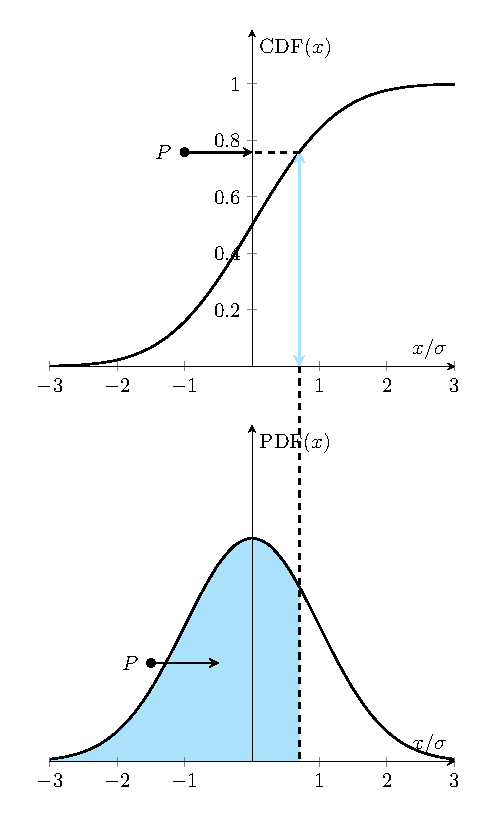
\includegraphics[width = 90mm]{Figures/figure-CDF.pdf}
    \caption{Sampling using an inverse CDF}
    \label{fig: CDF}
\end{figure}

The simplest method for sampling from a univariate distribution is based on the inverse probability transform. As shown in \cref{fig: CDF}, if we can get the cumulative probability density function, then we can easily generate samples by computing $x$ = CDF($\mathcal{U}$). $\mathcal{U}$ follows uniform distribution $\mathcal{U} \sim U(0,1)$.




\subsubsection{Rejection sampling}
When the inverse cdf method cannot be used, one simple alternative is to use rejection sampling. In rejection sampling, we create a proposal distribution $q(x)$ which satisfies $Mq(x) \geq \tilde{p}(x)$, for some constant $M$, where $\tilde{p}(x)$ is an unnormalized version of $p(x)$ (i.e., $p(x)$ = $\tilde{p}(x)/Z$ for some unknown constant $Z$). The function $Mq(x)$ provides an upper envelope for $\tilde{p}$. We then sample $x \sim q(x)$, which corresponds to picking a random $x$ location, and then we sample $u \sim U(0,1)$ which corresponds to picking a random height ($y$ location) under the
envelope. If $u \geq \frac{\tilde{p}(x)}{Mq(x)}$, we reject the sample,otherwise we accept it. See \cref{fig: rejectsampling}, where acceptance region is shown shaded, and the rejection region is the white region between the shaded zone and the upper envelope.
\begin{figure}[htbp]
    \centering
    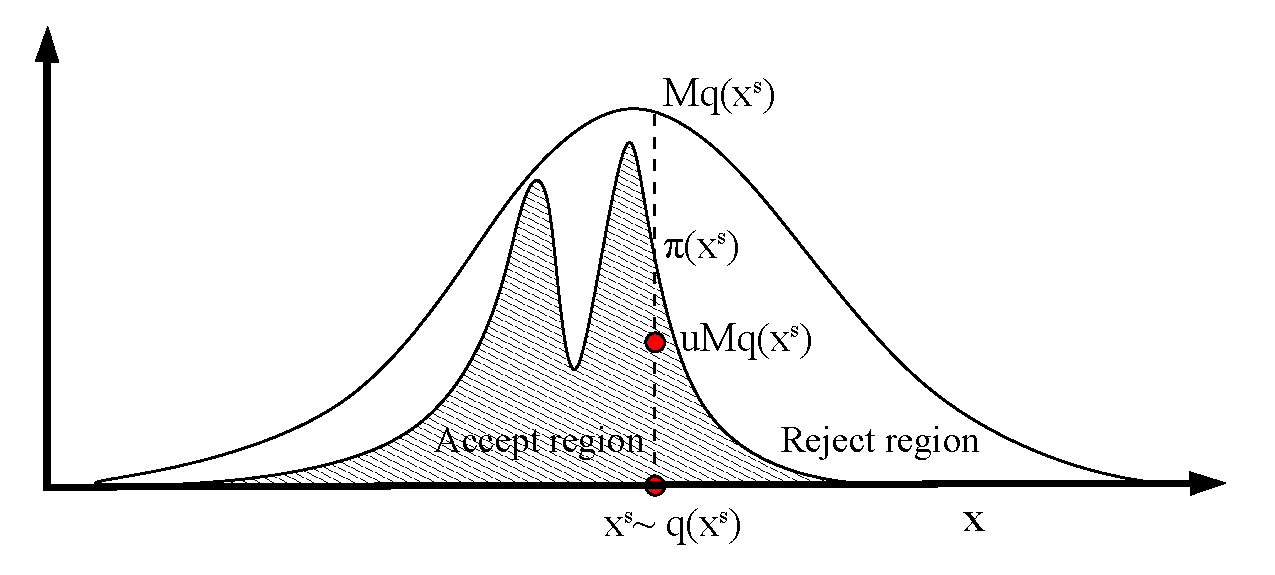
\includegraphics[width = 140mm]{Figures/figure-rejectionsampling.pdf}
    \caption{Schematic illustration of rejection sampling from \protect\cite{andrieu2003}}
    \label{fig: rejectsampling}
\end{figure}
But, large-dimensional spaces tend to be very empty, and the chances that this method accepts a point may be dramatically low when working with multidimensional spaces. \acrshort{MCMC}

\subsubsection{Importance sampling}

Often, in practical Bayesian models, it is not possible to obtain samples directly from p.x j y1WT / due to its complicated functional form.

\subsubsection{Sequential Monte Carlo}


\subsubsection{Markov chain Monte Carlo}

\acrshort{MCMC}
Some Monte Carlo methods, including rejection sampling, importance sampling and particle filtering. The trouble with these methods is that they do not work well in high
dimensional spaces. The most popular method for sampling from high-dimensional distributions
is Markov chain Monte Carlo or MCMC. In a survey by \textit{SIAM News}
, MCMC was placed in the
top 10 most important algorithms of the 20th century \citep{murphy2012}.
\begin{figure}[H]
    \centering
    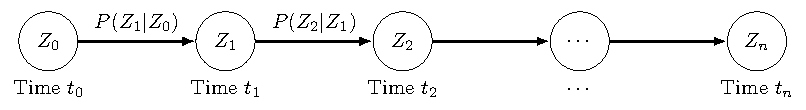
\includegraphics[width = 140mm]{Figures/figure-markov_process.pdf}
    \caption{Markov Chain process}
    \label{fig: markovchain}
\end{figure}


\subsection{Choice of sampling method}


\subsection{Seqential Bayesian inference}


\section{Sequential enrichment for surrogate model}

Traditional large-scale physics-based models are intractable to solve real-time, many-query context problem. 


Instead of sampling the whole experimental design at once, it has been proposed to use sequential enrichment. Starting with
a small experimental design, additional points are chosen based on the last computed sparse
solution. In the context of machine learning, sequential sampling is also known as active learning.  In all cases, numerical examples show that the sequential strategy generally leads to solutions with
a smaller validation error compared to non-sequential strategies

\section{Sensitivity analysis}